\documentclass[10pt]{article}
\usepackage[utf8]{inputenc}
\usepackage[T1]{fontenc}
\usepackage{amsmath}
\usepackage{amsfonts}
\usepackage{amssymb}
\usepackage[version=4]{mhchem}
\usepackage{stmaryrd}
\usepackage{graphicx}
\usepackage[export]{adjustbox}
\graphicspath{ {./images/} }

\title{PROBLEMS: }

\author{}
\date{}


\begin{document}
\maketitle
READING: Section 19.6 in Shankar on two particle scattering.

Some facts that might come in handy:


\begin{align*}
j_{\ell}(x) & =\sqrt{\frac{\pi}{2 x}} J_{\ell+\frac{1}{2}}(x)  \tag{1}\\
n_{\ell}(x) & =\sqrt{\frac{\pi}{2 x}} Y_{\ell+\frac{1}{2}}(x)  \tag{2}\\
h_{\ell}^{(1)}(x) & =\sqrt{\frac{\pi}{2 x}} H_{\ell+\frac{1}{2}}^{(1)}(x)  \tag{3}\\
J_{\nu}(x) & \sim \sqrt{\frac{2}{\pi x}} \cos \left(x-\nu \frac{\pi}{2}-\frac{\pi}{4}\right)  \tag{4}\\
H_{\nu}^{(1)}(x) & \sim \sqrt{\frac{2}{\pi x}} e^{i\left(x-\nu \frac{\pi}{2}-\frac{\pi}{4}\right)} . \tag{5}
\end{align*}


\begin{enumerate}
  \setcounter{enumi}{32}
  \item Show that the total cross section we computed in the partial wave expansion,
\end{enumerate}


\begin{equation*}
\sigma_{T}(p)=\frac{4 \pi}{p^{2}} \sum_{j=0}^{\infty}(2 j+1) \sin ^{2} \delta_{j}(p) \tag{6}
\end{equation*}


is in agreement with the optical theorem. That is, start with the optical theorem and derive the expression above.

\begin{enumerate}
  \setcounter{enumi}{33}
  \item We have discussed the "central force problem". Consider a particle of mass $m$ under the influence of the following potential:
\end{enumerate}

\[
V(r)= \begin{cases}V_{0}, & 0 \leq r \leq a  \tag{7}\\ 0, & a<r\end{cases}
\]

where $V_{0}$ is a constant.

(a) If $V_{0}<0$, what can you say about the phase shift, $\delta_{\ell}$, in partial wave $\ell$, for scattering on this potential. What if $V_{0}>0$ ? For $V_{0} \neq 0$ is it possible for the scattering amplitude in a given partial wave to vanish?

(b) Write down the Schrödinger equation for the wave function $\psi(\mathbf{x})$. Consider solutions which are simultaneous eigenvectors of $H, \mathbf{L}^{2}$, and $L_{z}$. Solve the angular dependence, and reduce the remaining problem to a problem in one variable.

(c) Let $E>0$ be an eigenvalue of the Hamiltonian, $H$. Solve the Schrödinger equation for eigenstates $\psi(\mathbf{x})$. It will probably be convenient to use the quantity $K=\sqrt{2 m\left(V_{0}-E\right)}$.

You may wish to express your solution for the phase shifts $\alpha_{\ell}$ in terms of the "logarithmic derivative".


\begin{equation*}
\left.L_{\ell} \equiv \frac{d \log j_{\ell}(i K r)}{d \log r}\right|_{x=a} \tag{8}
\end{equation*}


Hint: You will probably benefit by thinking about solutions in the form of spherical Bessel/Neumann functions, and/or spherical Hankel functions. See, e.g., section 12.6 of Shankar.

(d) Consider the limit as $r \rightarrow \infty$ for your solutions, and give an interpretation in terms of spherical waves.

\begin{enumerate}
  \setcounter{enumi}{34}
  \item Consider scattering from the simple potential:
\end{enumerate}

$$
V(\mathbf{x})= \begin{cases}V_{0} & r=|\mathbf{x}|<R \\ 0 & r>R\end{cases}
$$

In the low energy limit, we might only look at $S$-wave $\ell=0$ scattering. However, in the high energy limit, we expect scattering in other partial waves to become significant. For simplicity, let us here consider scattering on a hard sphere, $V_{0} \rightarrow \infty$.

(a) For a hard sphere potential, calculate the total cross section in partial wave $\ell$. Give the exact result, i.e., don't take the high energy limit yet. You may quote your answer in terms of the spherical Bessel functions.

(b) Find a simple expression for the phase shift $\delta_{\ell}$ in the high energy limit $(k R \gg$ $\ell$ ). Keep terms up to $\mathrm{O}(1)$ in your result.

(c) Determine the total cross section (including all partial waves) in the high energy limit, $k R \rightarrow \infty$. [This is the only somewhat tricky part of this problem to calculate. One approach is as follows: Write down the total cross section in terms of your results for part (a). Then, for fixed $k$, consider which values of $\ell$ may be important in the sum. Neglect the other values of $\ell$, and make the high energy approximation to your part (a) result. Finally, evaluate the sum, either directly, or by turning it into an appropriate integral.]

\begin{enumerate}
  \setcounter{enumi}{35}
  \item Consider the graph in Fig. 1. The numbers from which this graph was made are available in the file Delta++PhaseShifts.txt in the module for week 9.
\end{enumerate}

Assume that the other phase shifts are negligible (e.g., "low energy" is reasonably accurate). The pion mass and energy here are sufficiently small that we can at least entertain the approximation of an infinitely heavy proton at rest - we'll assume this to be the case, in any event. Note that $T_{\pi}$ is the relativistic kinetic energy of the $\pi^{+}: T_{\pi}=\sqrt{P_{\pi}^{2}+m_{\pi}^{2}}-m_{\pi}$.

(a) Is the $\pi^{+} p$ force principally attractive or repulsive (as shown in this figure)?

(b) Plot the total cross section in mb (millibarns) as a function of energy, from $T_{\pi}=40$ to $200 \mathrm{MeV}$.

(c) Plot the angular distribution of the scattered $\pi^{+}$at energies of 120, 140 and $160 \mathrm{MeV}$.

(d) What is the mean free path of $140 \mathrm{MeV}$ pions in a liquid hydrogen target, with these "protons"?

\begin{center}
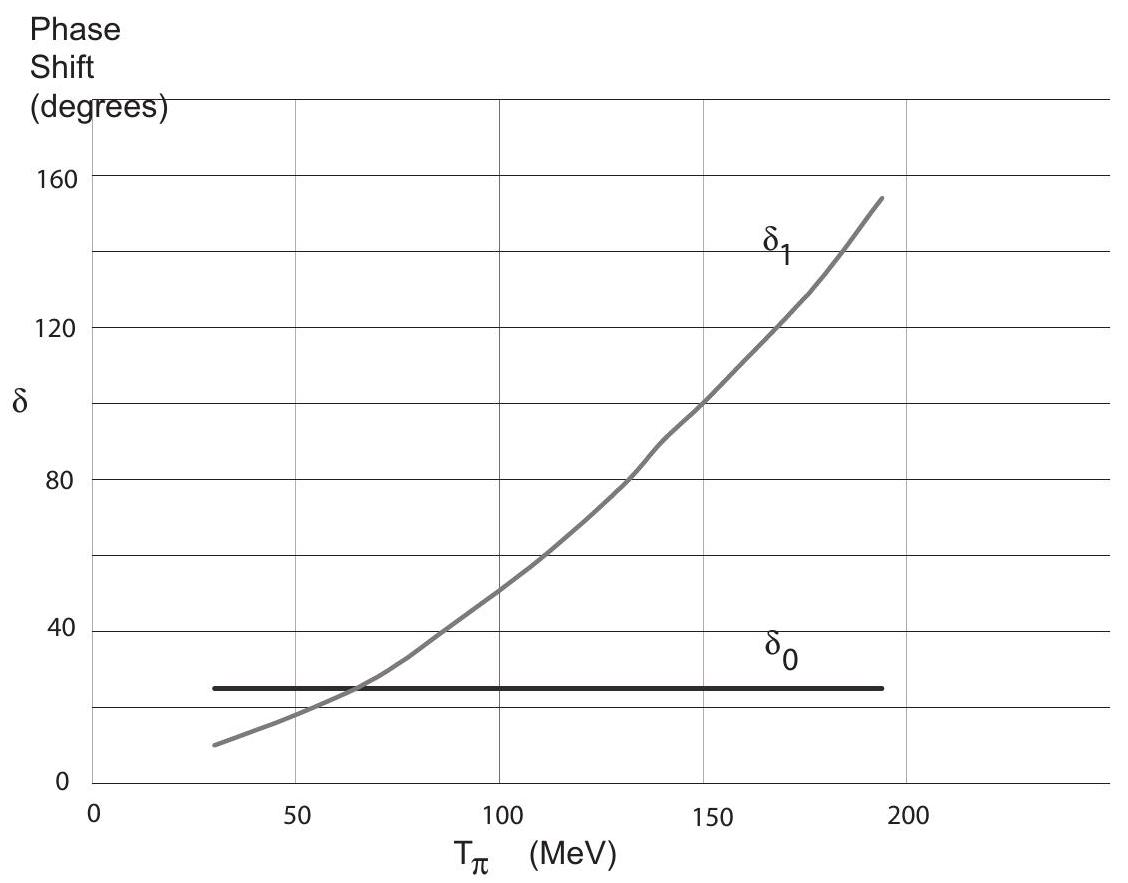
\includegraphics[max width=\textwidth]{2024_03_02_e4ccbaaa87e764c710bfg-3}
\end{center}

Figure 1: Made-up (but motivated by the famous " 33 resonance" in $\pi^{+} p$ scattering) graph of phase shifts $\delta_{0}$ and $\delta_{1}$ for elastic $\pi^{+} p$ scattering (neglecting spin).


\end{document}